\documentclass{standalone}
\usepackage{tikz}
\usetikzlibrary{patterns, positioning}
\usepackage[sfdefault]{ClearSans} %% option 'sfdefault' activates Clear Sans as the default text font
\usepackage[T1]{fontenc}

\begin{document}
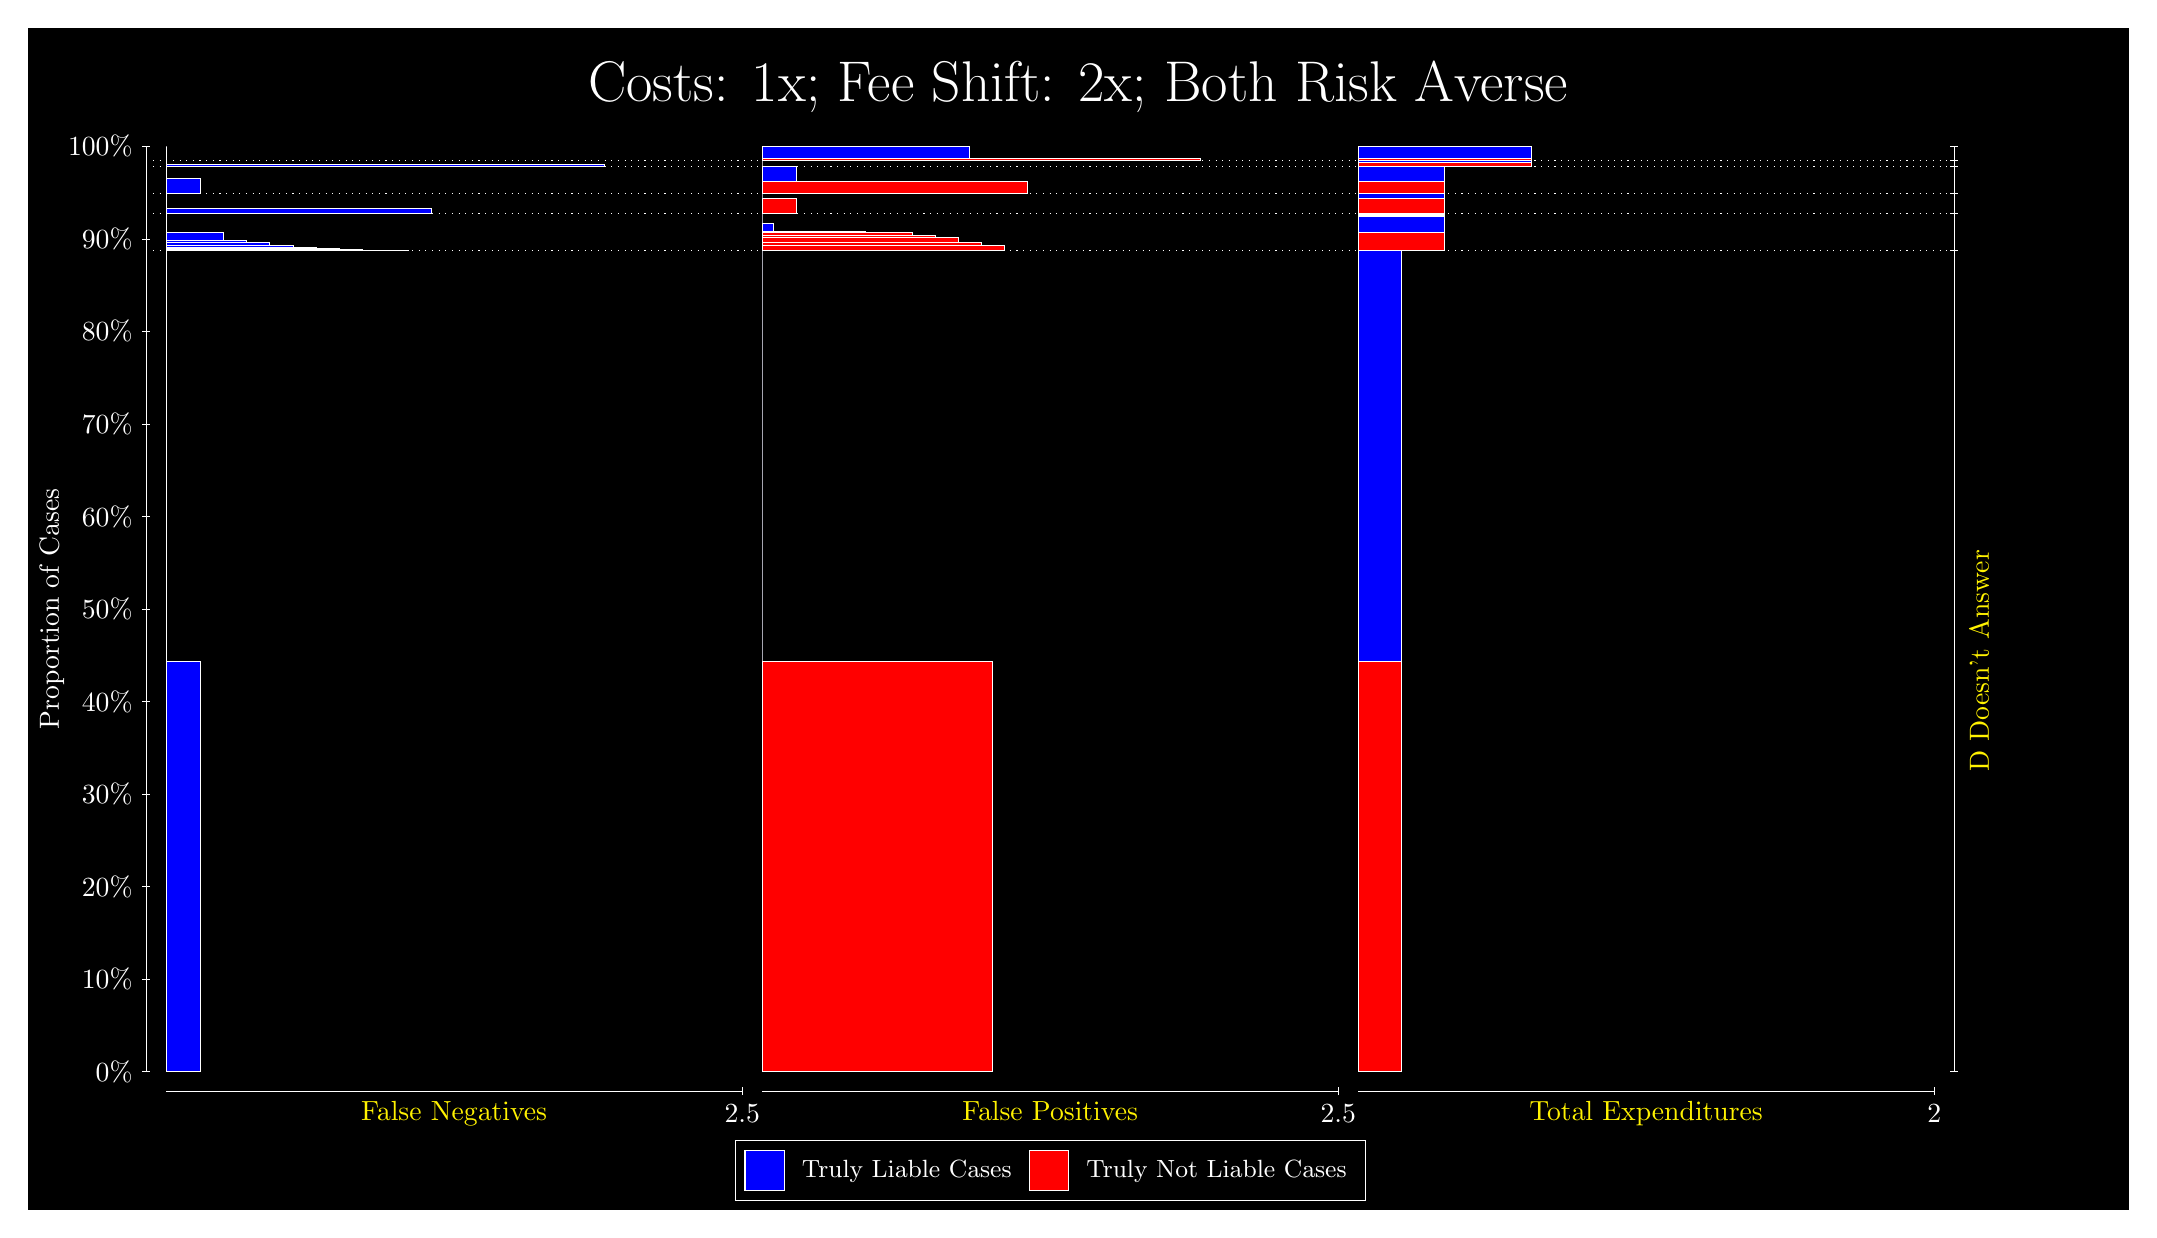
\begin{tikzpicture}
\draw[fill=black] (0,0) rectangle (26.667,15);
\draw[text=white] (0,13.5) rectangle (26.667,15) node[midway] {\huge Costs: 1x; Fee Shift: 2x; Both Risk Averse};
\draw[white, very thin] (1.5,1.75) -- (1.5,13.5);
\node[rotate=90, text=white, anchor=center] at (0.3, 7.625) {Proportion of Cases};
\draw[white, very thin] (1.45,1.75) -- (1.55,1.75);
\node[text=white, anchor=east] at (1.45, 1.75) {0\%};
\draw[white, very thin] (1.45,2.925) -- (1.55,2.925);
\node[text=white, anchor=east] at (1.45, 2.925) {10\%};
\draw[white, very thin] (1.45,4.1) -- (1.55,4.1);
\node[text=white, anchor=east] at (1.45, 4.1) {20\%};
\draw[white, very thin] (1.45,5.275) -- (1.55,5.275);
\node[text=white, anchor=east] at (1.45, 5.275) {30\%};
\draw[white, very thin] (1.45,6.45) -- (1.55,6.45);
\node[text=white, anchor=east] at (1.45, 6.45) {40\%};
\draw[white, very thin] (1.45,7.625) -- (1.55,7.625);
\node[text=white, anchor=east] at (1.45, 7.625) {50\%};
\draw[white, very thin] (1.45,8.8) -- (1.55,8.8);
\node[text=white, anchor=east] at (1.45, 8.8) {60\%};
\draw[white, very thin] (1.45,9.975) -- (1.55,9.975);
\node[text=white, anchor=east] at (1.45, 9.975) {70\%};
\draw[white, very thin] (1.45,11.15) -- (1.55,11.15);
\node[text=white, anchor=east] at (1.45, 11.15) {80\%};
\draw[white, very thin] (1.45,12.325) -- (1.55,12.325);
\node[text=white, anchor=east] at (1.45, 12.325) {90\%};
\draw[white, very thin] (1.45,13.5) -- (1.55,13.5);
\node[text=white, anchor=east] at (1.45, 13.5) {100\%};

\draw[white, very thin] (24.457,1.75) -- (24.457,13.5);
\draw[white, very thin] (24.407,1.75) -- (24.507,1.75);
\node[anchor=west] at (24.407, 1.75) {};
\draw[white, very thin] (24.407,12.18) -- (24.507,12.18);
\node[anchor=west] at (24.407, 12.18) {};
\draw[white, very thin] (24.407,12.647) -- (24.507,12.647);
\node[anchor=west] at (24.407, 12.647) {};
\draw[white, very thin] (24.407,12.906) -- (24.507,12.906);
\node[anchor=west] at (24.407, 12.906) {};
\draw[white, very thin] (24.407,13.244) -- (24.507,13.244);
\node[anchor=west] at (24.407, 13.244) {};
\draw[white, very thin] (24.407,13.324) -- (24.507,13.324);
\node[anchor=west] at (24.407, 13.324) {};
\draw[white, very thin] (24.407,13.5) -- (24.507,13.5);
\node[anchor=west] at (24.407, 13.5) {};

\draw[white, very thin, fill=blue] (1.75,1.75) rectangle (2.1891,6.9647);
\draw[white, very thin, fill=red] (1.75,6.9647) rectangle (1.75,12.18);
\draw[white, very thin, fill=blue] (1.75,12.18) rectangle (4.8239,12.183);
\draw[white, very thin, fill=blue] (1.75,12.183) rectangle (4.5312,12.186);
\draw[white, very thin, fill=blue] (1.75,12.186) rectangle (4.2384,12.193);
\draw[white, very thin, fill=blue] (1.75,12.193) rectangle (3.9457,12.2);
\draw[white, very thin, fill=blue] (1.75,12.2) rectangle (3.6529,12.22);
\draw[white, very thin, fill=blue] (1.75,12.22) rectangle (3.3602,12.238);
\draw[white, very thin, fill=blue] (1.75,12.238) rectangle (3.0674,12.277);
\draw[white, very thin, fill=blue] (1.75,12.277) rectangle (2.7746,12.302);
\draw[white, very thin, fill=blue] (1.75,12.302) rectangle (2.4819,12.404);
\draw[white, very thin, fill=red] (1.75,12.404) rectangle (1.75,12.647);
\draw[white, very thin, fill=blue] (1.75,12.647) rectangle (5.1167,12.715);
\draw[white, very thin, fill=red] (1.75,12.715) rectangle (1.75,12.906);
\draw[white, very thin, fill=blue] (1.75,12.906) rectangle (2.1891,13.099);
\draw[white, very thin, fill=red] (1.75,13.099) rectangle (1.75,13.244);
\draw[white, very thin, fill=blue] (1.75,13.244) rectangle (7.3123,13.27);
\draw[white, very thin, fill=red] (1.75,13.27) rectangle (1.75,13.324);
\draw[white, very thin, fill=red] (1.75,13.324) rectangle (1.75,13.351);
\draw[white, very thin, fill=blue] (1.75,13.351) rectangle (1.75,13.5);
\draw[white, very thin, fill=red] (9.3189,1.75) rectangle (12.246,6.9649);
\draw[white, very thin, fill=blue] (9.3189,6.9649) rectangle (9.3189,12.18);
\draw[white, very thin, fill=red] (9.3189,12.18) rectangle (12.393,12.243);
\draw[white, very thin, fill=red] (9.3189,12.243) rectangle (12.1,12.276);
\draw[white, very thin, fill=red] (9.3189,12.276) rectangle (11.807,12.34);
\draw[white, very thin, fill=red] (9.3189,12.34) rectangle (11.515,12.374);
\draw[white, very thin, fill=red] (9.3189,12.374) rectangle (11.222,12.406);
\draw[white, very thin, fill=red] (9.3189,12.406) rectangle (10.929,12.409);
\draw[white, very thin, fill=red] (9.3189,12.409) rectangle (10.929,12.412);
\draw[white, very thin, fill=red] (9.3189,12.412) rectangle (10.636,12.418);
\draw[white, very thin, fill=red] (9.3189,12.418) rectangle (10.344,12.42);
\draw[white, very thin, fill=red] (9.3189,12.42) rectangle (10.051,12.423);
\draw[white, very thin, fill=blue] (9.3189,12.423) rectangle (9.4652,12.525);
\draw[white, very thin, fill=blue] (9.3189,12.525) rectangle (9.3189,12.647);
\draw[white, very thin, fill=red] (9.3189,12.647) rectangle (9.758,12.838);
\draw[white, very thin, fill=blue] (9.3189,12.838) rectangle (9.3189,12.906);
\draw[white, very thin, fill=red] (9.3189,12.906) rectangle (12.686,13.051);
\draw[white, very thin, fill=blue] (9.3189,13.051) rectangle (9.758,13.244);
\draw[white, very thin, fill=red] (9.3189,13.244) rectangle (9.3189,13.299);
\draw[white, very thin, fill=blue] (9.3189,13.299) rectangle (9.3189,13.324);
\draw[white, very thin, fill=red] (9.3189,13.324) rectangle (14.881,13.351);
\draw[white, very thin, fill=blue] (9.3189,13.351) rectangle (11.954,13.5);
\draw[white, very thin, fill=red] (16.888,1.75) rectangle (17.437,6.9649);
\draw[white, very thin, fill=blue] (16.888,6.9649) rectangle (17.437,12.18);
\draw[white, very thin, fill=red] (16.888,12.18) rectangle (17.986,12.409);
\draw[white, very thin, fill=blue] (16.888,12.409) rectangle (17.986,12.617);
\draw[white, very thin, fill=red] (16.888,12.617) rectangle (17.986,12.619);
\draw[white, very thin, fill=blue] (16.888,12.619) rectangle (17.986,12.623);
\draw[white, very thin, fill=red] (16.888,12.623) rectangle (17.986,12.634);
\draw[white, very thin, fill=blue] (16.888,12.634) rectangle (17.986,12.647);
\draw[white, very thin, fill=red] (16.888,12.647) rectangle (17.986,12.838);
\draw[white, very thin, fill=blue] (16.888,12.838) rectangle (17.986,12.906);
\draw[white, very thin, fill=red] (16.888,12.906) rectangle (17.986,13.051);
\draw[white, very thin, fill=blue] (16.888,13.051) rectangle (17.986,13.244);
\draw[white, very thin, fill=red] (16.888,13.244) rectangle (19.083,13.299);
\draw[white, very thin, fill=blue] (16.888,13.299) rectangle (19.083,13.324);
\draw[white, very thin, fill=red] (16.888,13.324) rectangle (19.083,13.351);
\draw[white, very thin, fill=blue] (16.888,13.351) rectangle (19.083,13.5);
\draw[white, dotted] (1.5,12.18) -- (24.457,12.18);
\draw[white, dotted] (1.5,12.647) -- (24.457,12.647);
\draw[white, dotted] (1.5,12.906) -- (24.457,12.906);
\draw[white, dotted] (1.5,13.244) -- (24.457,13.244);
\draw[white, dotted] (1.5,13.324) -- (24.457,13.324);
\draw[white, very thin] (1.75,1.5) -- (9.0689,1.5);
\node[text=yellow, anchor=north] at (5.4094, 1.5) {False Negatives};
\draw[white, very thin] (9.0689,1.45) -- (9.0689,1.55);
\node[text=white, anchor=north] at (9.0689, 1.45) {2.5};

\draw[white, very thin] (9.3189,1.5) -- (16.638,1.5);
\node[text=yellow, anchor=north] at (12.978, 1.5) {False Positives};
\draw[white, very thin] (16.638,1.45) -- (16.638,1.55);
\node[text=white, anchor=north] at (16.638, 1.45) {2.5};

\draw[white, very thin] (16.888,1.5) -- (24.207,1.5);
\node[text=yellow, anchor=north] at (20.547, 1.5) {Total Expenditures};
\draw[white, very thin] (24.207,1.45) -- (24.207,1.55);
\node[text=white, anchor=north] at (24.207, 1.45) {2};

\node[text=yellow, centered, rotate=90] at (24.777, 6.9648) {D Doesn't Answer};






\draw (12.978300999999998,1.5) node[draw=none] (baseCoordinate) {};
\begin{scope}[align=center]
        \matrix[scale=0.5, draw=white, below=0.5cm of baseCoordinate, nodes={draw}, column sep=0.1cm]{
            \node[rectangle, draw, minimum width=0.5cm, minimum height=0.5cm, fill=blue] {}; &
            \node[draw=none, font=\small, text=white] (B) {Truly Liable Cases}; &
            \node[rectangle, draw, minimum width=0.5cm, minimum height=0.5cm, fill=red] {}; &
            \node[draw=none, font=\small, text=white] (B) {Truly Not Liable Cases}; \\
            };
\end{scope}

\end{tikzpicture}
\end{document}